\documentclass[xcolor=pst,dvips,12pt,english,french]{beamer}
\usepackage[backend=biber,style=numeric,firstinits=true, isbn=false, url=false, doi=false, eprint=false]{biblatex}

\bibliography{../biblio3.bib}
\usepackage{graphicx}
\usepackage{babel}
\usepackage[utf8]{inputenc}
\usepackage{lmodern}
\usepackage{beamerthemeshadow}
\usepackage[skip=2pt,font=scriptsize,labelformat=empty]{caption} % Required for specifying captions to tables and figures
\usepackage{pstricks}

\title{Apprendre par synchronie ?}
\author{Fournier Pierre}

\newrobustcmd*{\footlessfullcite}{\AtNextCite{\renewbibmacro{title}{}\renewbibmacro{in:}{}}\footfullcite}


\begin{document}
	\frame{\titlepage} 
	
	%\frame{\frametitle{Table of contents}\tableofcontents} 
	
	\begin{frame}{Objectifs}
		Etant donné un robot \textbf{autonome} en présence d'êtres humains, comment ces derniers peuvent susciter et guider l'apprentissage de \textbf{nouveaux comportements} par leur \textbf{interaction naturelle} avec le robot ?
		
		Deux cadres applicatifs :
		\begin{itemize}
			\item Personnalisation d'un robot de compagnie : apprentissage de jeux
			\item Spécialisation d'un robot industriel : apprentissage de tâches
		\end{itemize}
		Pas de compétence informatique requise.
	
	\end{frame}
	
	\begin{frame}{Approche choisie}
		\begin{columns}
			\begin{column}{0.55\textwidth}
				\includegraphics[width=\textwidth]{images/playroom.eps}
			\end{column}
			\begin{column}{0.45\textwidth}
				\begin{itemize}
					\item Robot modélisé par son attention et ses actions
					\item Le tuteur intervient par son attention
					\item But : orienter l'exploration autonome du robot vers une variation précise de la tâche (ex: blocs d'une couleur dans la boîte de la même couleur)
				\end{itemize}
			\end{column}
		\end{columns}
	\end{frame}
	
	\section{Exploration autonome}
	
	\begin{frame}{L'exploration autonome }
		But : découverte de séquences d'interactions pertinentes avec son environnement. 
		Solution classique : Reinforcement learning, avec récompenses définies pour unedécouverte de séquences d'interactions pertinentes avec son environnement.  tâche.
		Problème : plus les récompenses sont spécifiques, moins les compétences sont génériques.
		Solution : Motivation intrinsèque, le robot définit lui-même et s'attribue des objectifs définissant ses récompenses, selon un principe indépendant de toute tâche (goal-babbling, curiosité artificielle...)
		Le comportement exploratoire autonome du robot émerge de ce couplage entre RL et motivation intrinsèque, sans nécessité de récompenses ad hoc prédéfinies.
		Références.
	\end{frame}
	\begin{frame}{Exploration autonome}
		Objectif : découverte de séquences d'interactions pertinentes avec son environnement.
		
		Solution classique : RL. Des états de l'environnements sont "récompensants" et l'agent cherche un comportement décisionnel maximisant la récompense espérée.
		
		\begin{columns}
			\begin{column}{0.45\textwidth}
				\centering
				\includegraphics[width=\textwidth]{images/RL1.eps}
			\end{column}
			\begin{column}{0.5\textwidth}
				L'environnement ne fournit pas de récompense, et les définir a priori réduit l'adaptabilité du robot.
			\end{column}
		\end{columns}
	\end{frame}
	
	\begin{frame}{Motivation intrinsèque}
		Solution : Motivation intrinsèque, le robot définit lui-même et s'attribue des objectifs définissant ses récompenses, selon un principe indépendant de toute tâche (goal-babbling, curiosité artificielle...)
		
		Le comportement exploratoire autonome du robot émerge de ce couplage entre RL et motivation intrinsèque, sans nécessité de récompenses ad hoc prédéfinies.
		Références.
	\end{frame}
	
	\begin{frame}{Application au cadre expérimental}
		Obect centered selection of actions
		
		??????????
	\end{frame}
	
	\begin{frame}{Guidage de l'apprentissage vers une tâche spécifique}
		Contexte : le robot interagit avec l'environnement selon un mécanisme non spécifique à une tâche.
		Objectif : faire découvrir et valoriser la tâche souhaitée par le tuteur.
		Hypothèse : la qualité de l'interaction (= degré de synchronie spatio-temporelle, joint engagement) est valorisée intrinsèquement et très tôt par les enfants. 
		Exploitation de l'hypothèse : faire de cette qualité une origine de renforcement supplémentaire (comment ?) et observer les effets sur l'orientation de l'apprentissage.
	\end{frame}
	
	\begin{frame}{Related work}
		Interactive machine learning : imitation d'une démonstration, suivi d'une instruction. Requiert un protocole prédéfini d'apprentissage, l'interaction n'est qu'un moyen.
		
		Distinction labeled unlabeled guidance : le robot doit extraire une interprétation non évidente de l'interaction. Comment deviner que tel geste de la main est un renforcement ? Chez nous, l'interprétation est un side effect de l'amélioration de la qualité ? Modèle bayésien de l'interprétation chez Anis, chez nous l'interprétation est intégrée au protocole de découverte par RL ?
		
		Motivation par l'interaction : rythme comme motivation (Gaussier), imitation par la synchronie temporelle. Nous synchronie plus générale potentiellement.
	\end{frame}
	
	\begin{frame}{La robotique développementale}
		\begin{block}{Un robot peut-il apprendre comme un enfant ?}
			 Privilégier l'apprentissage de compétences bas niveau et mettre en place une architecture structurée permettant la progression autonome.
		\end{block}
		\begin{columns}
			\begin{column}{0.45\textwidth}
				\begin{exampleblock}{Contraintes}
					\begin{itemize}
						\item \emph{Lifelong learning}
						\item \emph{task-independent architecture}
						\item Complexité croissante des compétences
					\end{itemize}
				\end{exampleblock}
			\end{column}
			\begin{column}{0.45\textwidth}
				\begin{exampleblock}{Inspiration}
					Psychologie développementale, neurosciences, linguistique, biologie évolutionnaire...
				\end{exampleblock}
			\end{column}
		\end{columns}
	\end{frame}
	
	\begin{frame}{Interagir avec un environnement}
		\begin{block}{Embodied, situated robots}
			La cognition émerge chez un organisme par l'interaction avec son environnement, dépendante des capacités sensorimotrices de l'organisme dans cet environnement.
		\end{block}
		\begin{columns}
			\begin{column}{0.55\textwidth}
				\begin{exampleblock}{Autonomous object discovery}
					Interaction avec des objets : 
					\begin{itemize}
						\item Identification
						\item Apprentissage d'affordances
						\item Séquences d'actions
					\end{itemize}
				\end{exampleblock}
			\end{column}
			\begin{column}{0.35\textwidth}
				\vspace{0.5cm}
				\centering
				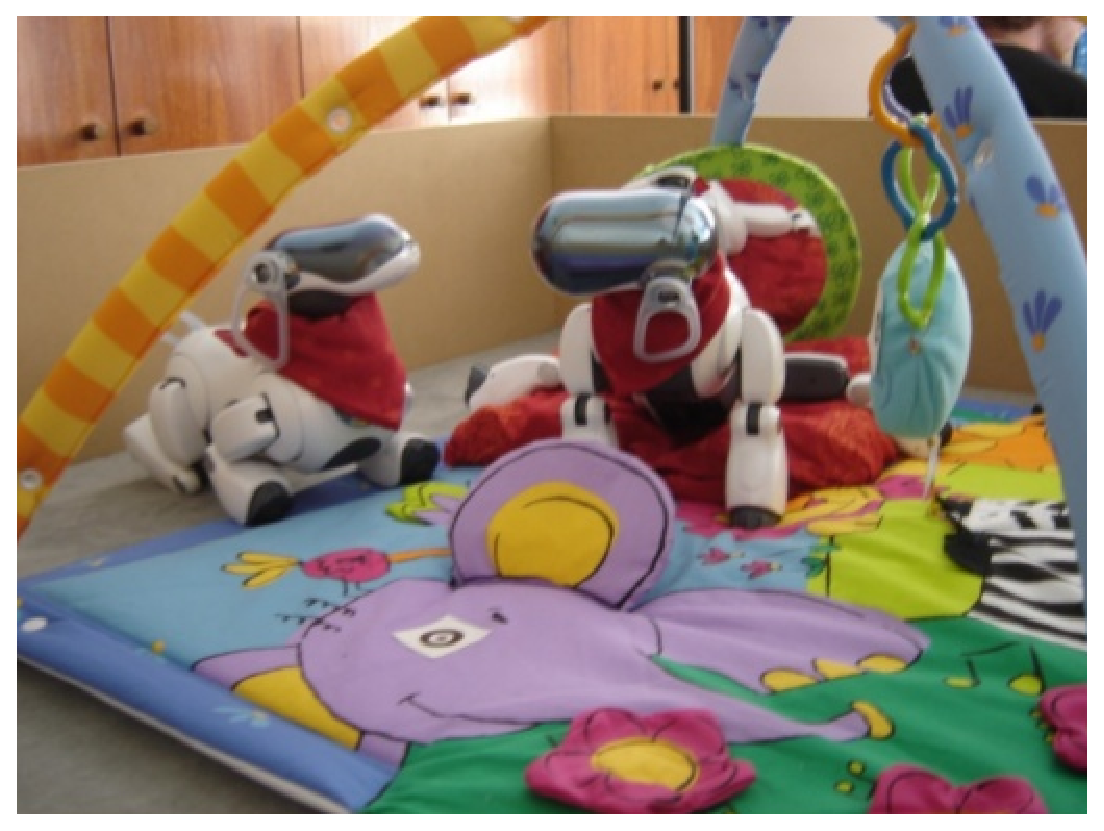
\includegraphics[width=\textwidth]{images/playground.eps}
				\captionof{figure}{The playground experiment}
			\end{column}
		\end{columns}
	\end{frame}
	
	\subsection{Intrinsically motivated reinforcement learning}
	
	
	
	\section{Positionnement de la thèse}

	\begin{frame}{Positionnement de la thèse}
		\begin{block}{Guidage de l'exploration}
			Au sein d'une tâche de découverte autonome d'un environnement, comment guider et accélérer l'exploration du robot par une interaction avec un tuteur humain ?
		\end{block}
		\begin{exampleblock}{Applications hors apprentissage développemental}
			Personnalisation / amélioration des compétences d'un robot de manière naturelle et sans recourir à la programmation.
			 \\ 
			$\to\,$ Jeu avec un robot de compagnie par exemple.
		\end{exampleblock}
	\end{frame}
	
	\subsection{Interactive reinforcement learning}
	
	\begin{frame}{Interactive reinforcement learning}
		\begin{block}{Principe}
			La récompense provient partiellement d'une interaction en temps réel avec un tuteur (démonstration, guidage,...)
		\end{block}
		\begin{exampleblock}{Labeled to unlabeled guidance}
			L'interprétation de l'interaction n'a pas de raison d'être connue du robot :
			\begin{itemize}
				\item Apprentissage de la tâche 
				\item Apprentissage du sens de l'interaction
			\end{itemize}
		\end{exampleblock}
	\end{frame}
	
	\begin{frame}{Réflexion sur l'interaction}
		\begin{block}{Constat chez les enfants}
			L'interaction elle-même semble être valorisée indépendamment de son objet : aide spontanée, reproduction d'un jeu une fois appris, etc.
		\end{block}
		\begin{exampleblock}{But des expériences futures}
			En attribuant au sein du mécanisme de motivation intrinsèque une valeur positive à la synchronie entre agent et tuteur, est-il possible de guider l'exploration autonome dans la direction manifestée par les actions du tuteur ? 
		\end{exampleblock}
	\end{frame}
	
	\subsection{Cadre actuel}
	
	\begin{frame}{Cadre de travail actuel}
		\begin{columns}
			\begin{column}{0.55\textwidth}
				\includegraphics[width=\textwidth]{images/playroom.eps}
			\end{column}
			\begin{column}{0.45\textwidth}
				\begin{block}{Synchrony-based guidance ?}
					\begin{itemize}
						\item Espace discrétisé
						\item Agent \& Tuteur : regard, intention, action
						\item Des boîtes et des blocs à ranger
						\item Un interrupteur nécessaire pour distinguer les couleurs
					\end{itemize}
				\end{block}
			\end{column}
		\end{columns}
	\end{frame}

\end{document}